\section{Flæðirit og sauðakóði}
\begin{figure}[h]
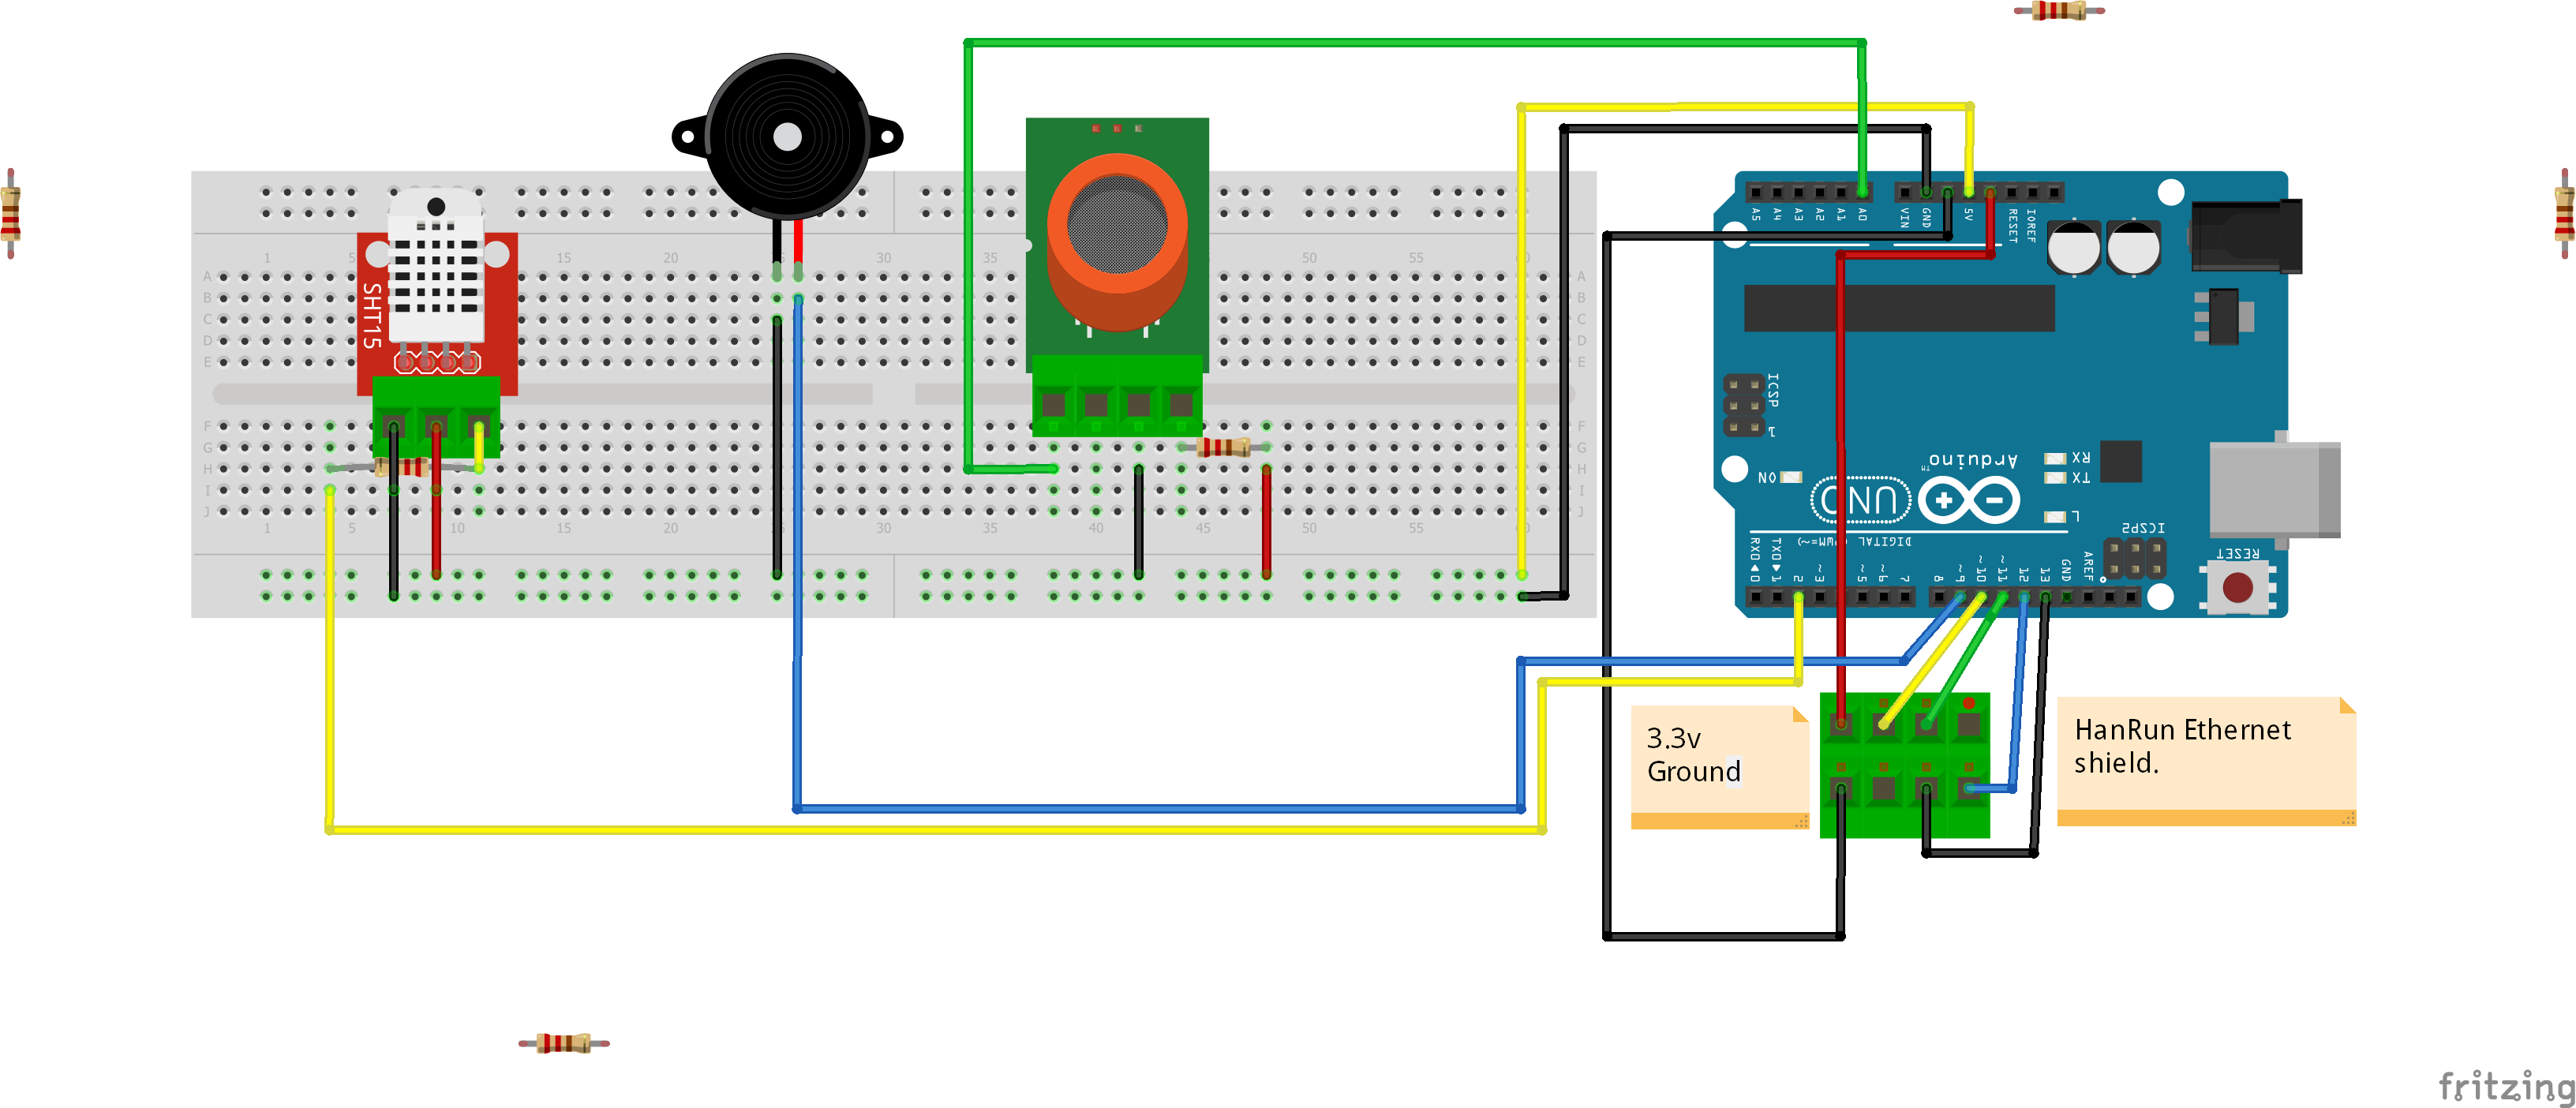
\includegraphics[scale=.4]{img/project}
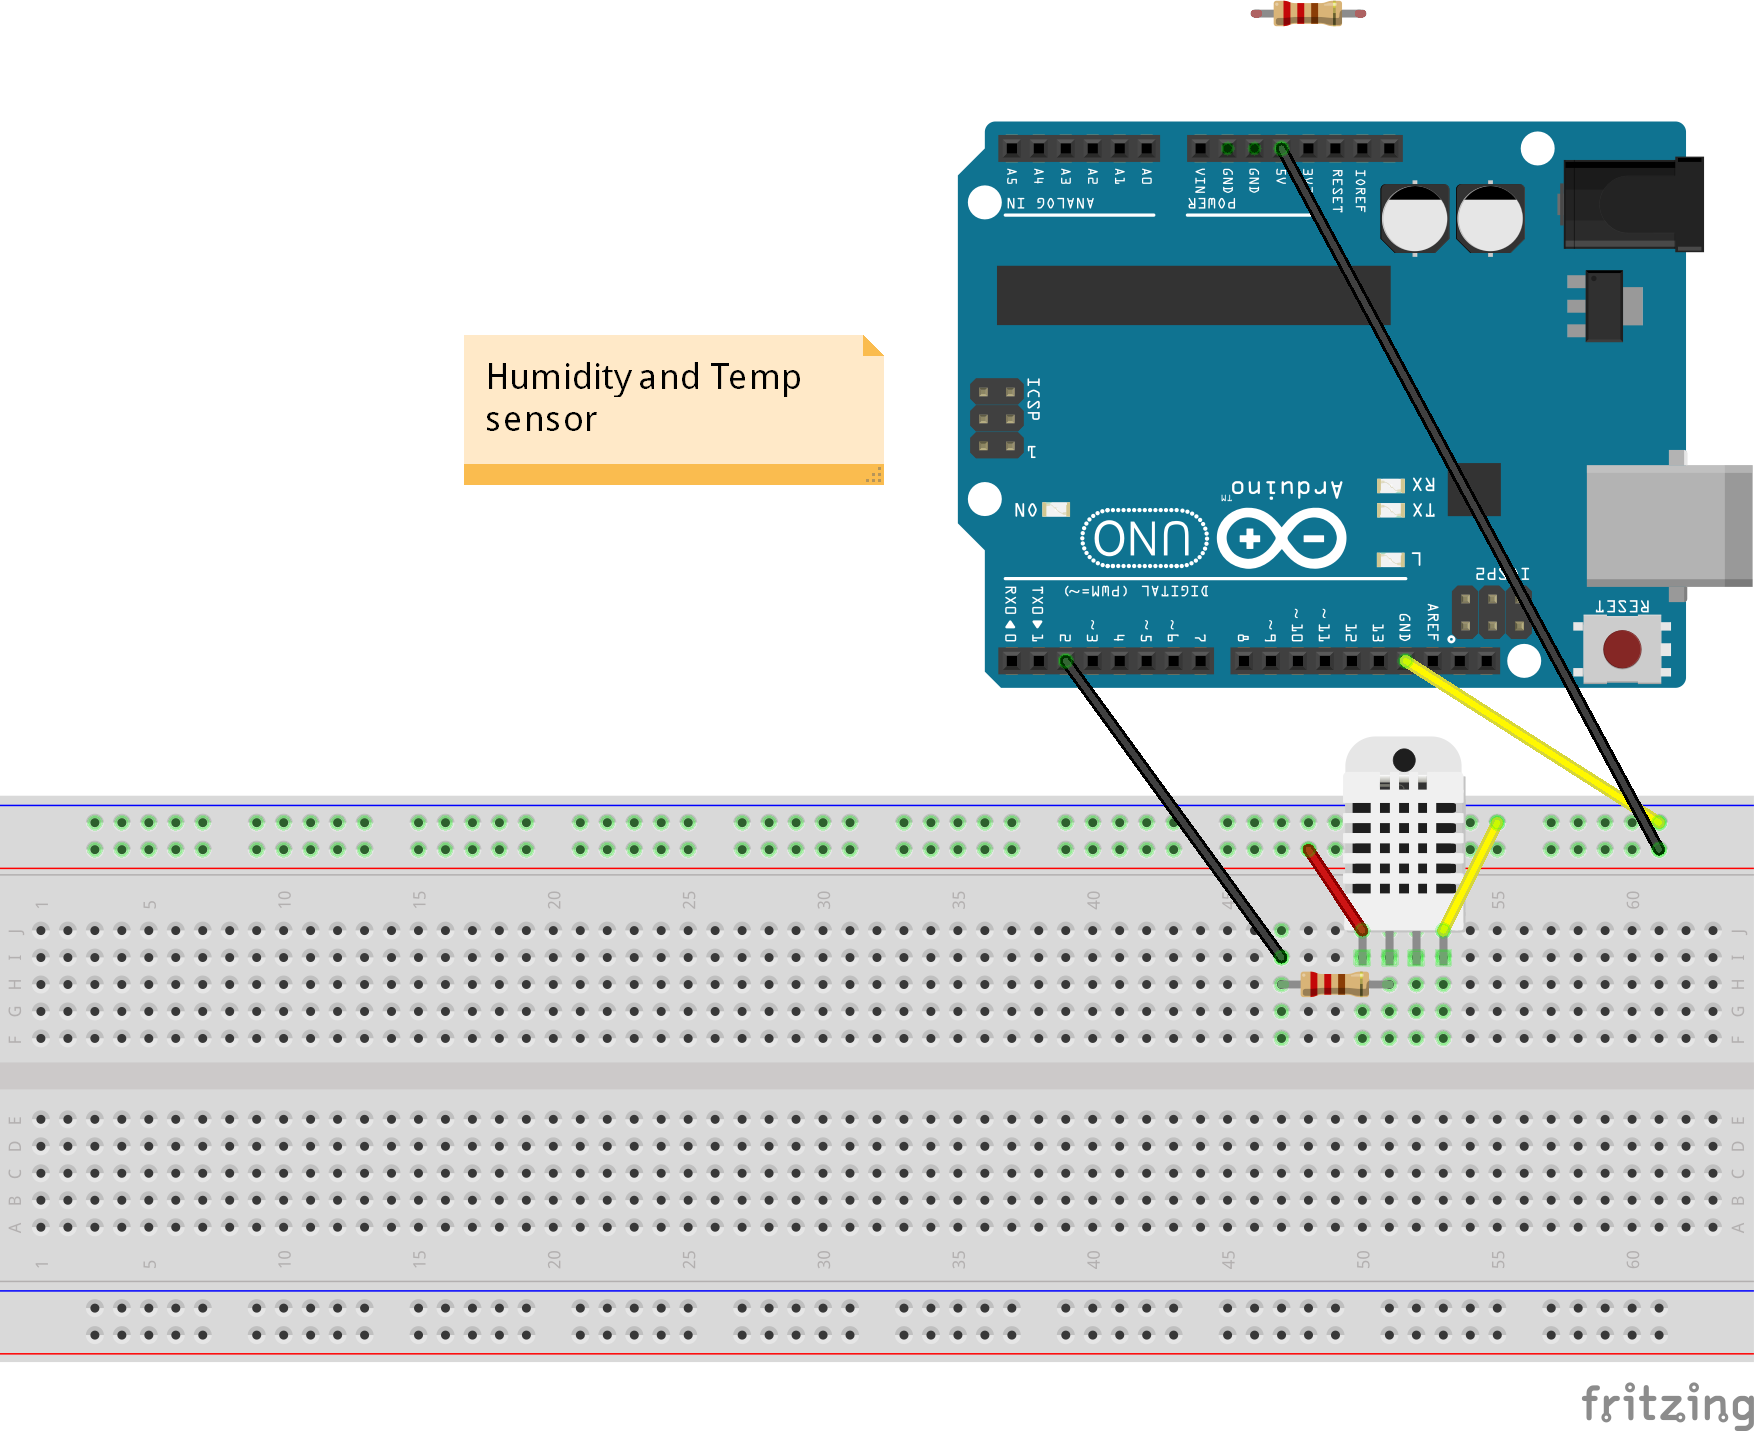
\includegraphics[scale=.4]{img/Humi_temp_bb} 
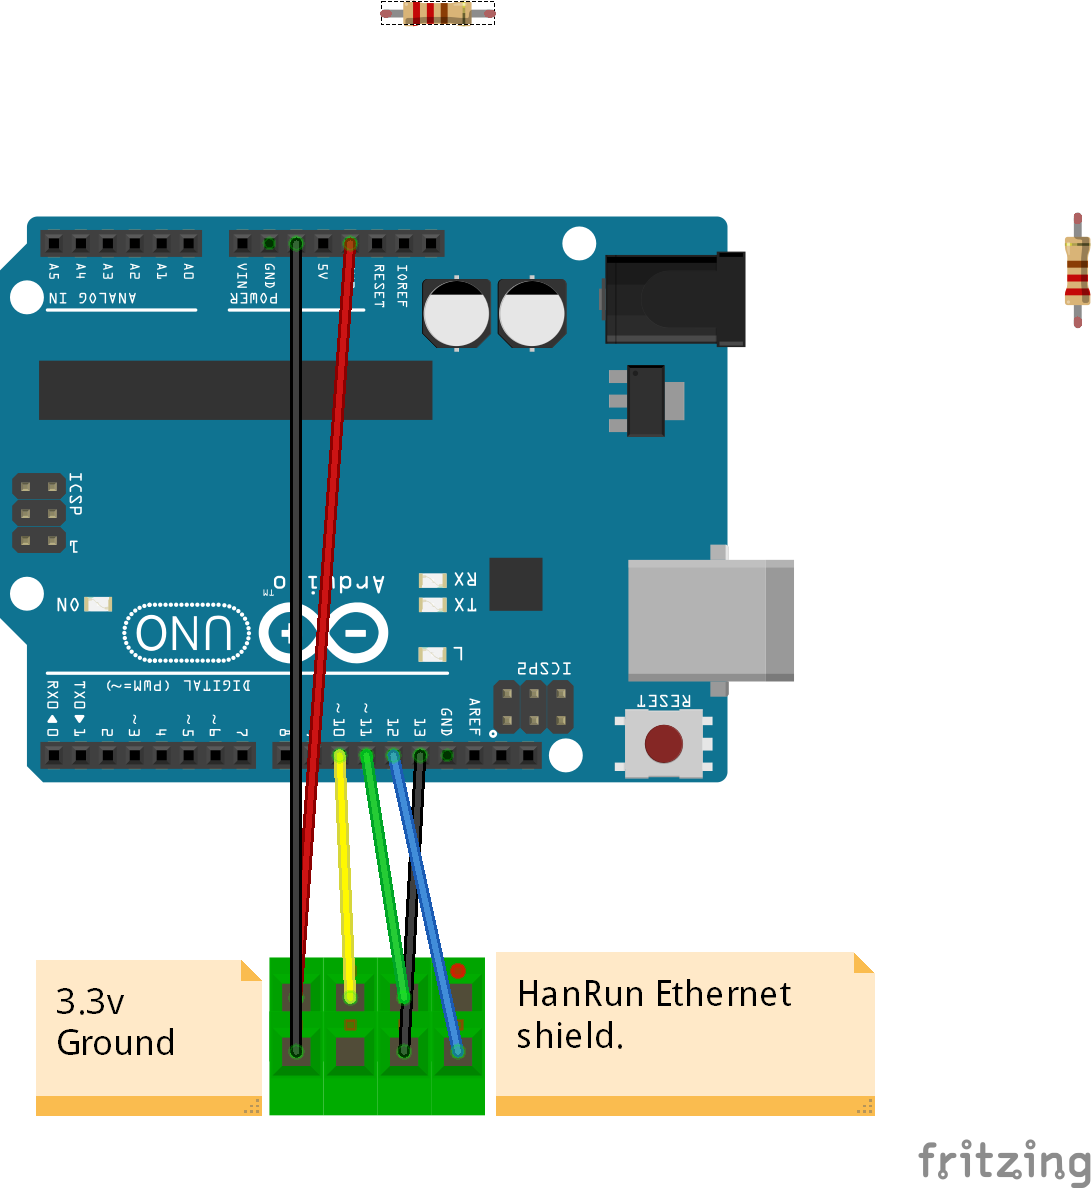
\includegraphics[scale=.5]{img/ethernet2}
\end{figure}
Verkefnið virkar þannig að það á að mæla hita, humitity og CO2 í loftinu.\\
Hitamælir:\\
void loop()\{
	int heat = heat-read();\\
	int temp = temp-read();\\

	Serial.print('heat);\\
	Serial.print('temp');\\
\}

MQ7 mælir: \\
int gasInn = 10;\\
int gasOut = A3;\\
void loop() \{
	get info from sensors\\
	Serial.println(sensorReading);\\
	Serial.println(gasAnalogReading);\\
\}
